%%%%%%%%%%%%%%%%%%%%%%%%%%%%%%%%%%%%%%%%%
% Short Sectioned Assignment
% LaTeX Template
% Version 1.0 (5/5/12)
%
% This template has been downloaded from:
% http://www.LaTeXTemplates.com
%
% Original author:
% Frits Wenneker (http://www.howtotex.com)
%
% License:
% CC BY-NC-SA 3.0 (http://creativecommons.org/licenses/by-nc-sa/3.0/)
%
%%%%%%%%%%%%%%%%%%%%%%%%%%%%%%%%%%%%%%%%%

%----------------------------------------------------------------------------------------
%	PACKAGES AND OTHER DOCUMENT CONFIGURATIONS
%----------------------------------------------------------------------------------------

\documentclass[paper=a4, fontsize=11pt]{scrartcl} % A4 paper and 11pt font size

\usepackage[T1]{fontenc} % Use 8-bit encoding that has 256 glyphs
\usepackage[utf8]{inputenc}
\usepackage[spanish]{babel} % English language/hyphenation
\usepackage{amsmath,amsfonts,amsthm} % Math packages
\usepackage{breakcites}
\usepackage{sectsty} % Allows customizing section commands
\allsectionsfont{\centering \normalfont\scshape} % Make all sections centered, the default font and small caps
\usepackage{algorithm}
\usepackage{url}
\usepackage[noend]{algpseudocode}
\makeatletter
\usepackage{graphicx}
\usepackage{listings}
\usepackage{color}
\usepackage{fancyhdr} % Custom headers and footers
\pagestyle{fancyplain} % Makes all pages in the document conform to the custom headers and footers
\fancyhead{} % No page header - if you want one, create it in the same way as the footers below
\fancyfoot[L]{} % Empty left footer
\fancyfoot[C]{} % Empty center footer
\fancyfoot[R]{\thepage} % Page numbering for right footer
\renewcommand{\headrulewidth}{0pt} % Remove header underlines
\renewcommand{\footrulewidth}{0pt} % Remove footer underlines
\setlength{\headheight}{13.6pt} % Customize the height of the header
% Reinsert missing \algbackskip
\def\algbackskip{\hskip-\ALG@thistlm}
\renewcommand*{\ALG@name}{Algoritmo}
\makeatother
\decimalpoint
\numberwithin{equation}{section} % Number equations within sections (i.e. 1.1, 1.2, 2.1, 2.2 instead of 1, 2, 3, 4)
\numberwithin{figure}{section} % Number figures within sections (i.e. 1.1, 1.2, 2.1, 2.2 instead of 1, 2, 3, 4)
\numberwithin{table}{section} % Number tables within sections (i.e. 1.1, 1.2, 2.1, 2.2 instead of 1, 2, 3, 4)

\setlength\parindent{0pt} % Removes all indentation from paragraphs - comment this line for an assignment with lots of text

%----------------------------------------------------------------------------------------
%	TITLE SECTION
%----------------------------------------------------------------------------------------

\newcommand{\horrule}[1]{\rule{\linewidth}{#1}} % Create horizontal rule command with 1 argument of height

\title{	
\normalfont \normalsize 
\textsc{Universidad Nacional de San Agustín, Escuela de ..} \\ [25pt] % Your university, school and/or department name(s)
\horrule{0.5pt} \\[0.4cm] % Thin top horizontal rule
\huge Árbol AVL \\ % The assignment title
\horrule{2pt} \\[0.5cm] % Thick bottom horizontal rule
}

\author{Christian E. Portugal Zambrano} % Your name

\date{\normalsize\today} % Today's date or a custom date

\begin{document}

\maketitle % Print the title

%----------------------------------------------------------------------------------------
%	PROBLEM 1
%----------------------------------------------------------------------------------------

\section{Introducción}
Los árboles de búsqueda binarios son árboles binarios en orden simétrico, cada nodo tiene una llave y cada llave del nodo puede ser mayor que todas las llaves en su sub-árbol izquierdo o menor que todas las llaves de su sub-árbol derecho, también un árbol binario puede estar vacío o formado por dos sub-árboles disjuntos. \\Un problema de los árboles de búsqueda binarios es la forma de inserción y borrado, de acuerdo a esto algunos árboles tienden a desnaturalizarse o perder sus propiedades de búsqueda. En este trabajo implementamos un árbol AVL que agrega un comportamiento de balanceo de nodos a los árboles de búsqueda ordinarios para resolver el problema de inserción y borrado.

%------------------------------------------------

\subsection{Árboles binarios de búsqueda}
Descrito anteriormente los árboles de búsqueda binarios dependen en cierto modo de la forma de inserción de sus llaves si existe un orden en los datos el árbol se visualiza y comporta como una lista enlazada, este es el peor de los casos, sin embargo en \cite{reed2000} se propone que si N llaves distintas son insertadas aleatoriamente en un árbol binarios de búsqueda, la altura esperada del árbol es $\sim 4.311 \ln N$  pero en el peor de los casos la altura es $N$. En la \figurename~\ref{fig:bst} se muestra árboles de búsqueda binaria balanceados (a) y no balanceados (b).
\begin{figure}[h]
	\begin{tabular}{cc}
		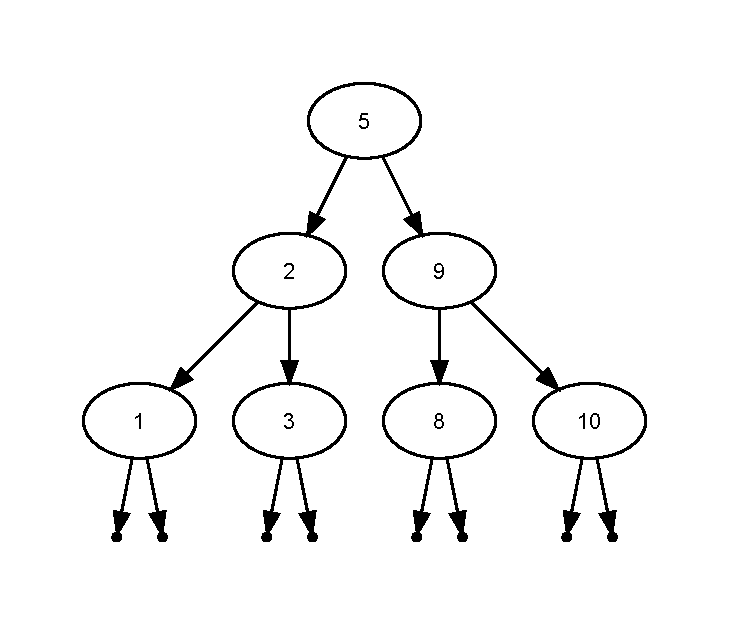
\includegraphics[width=0.5\textwidth,height=5cm]{balanced} & 
		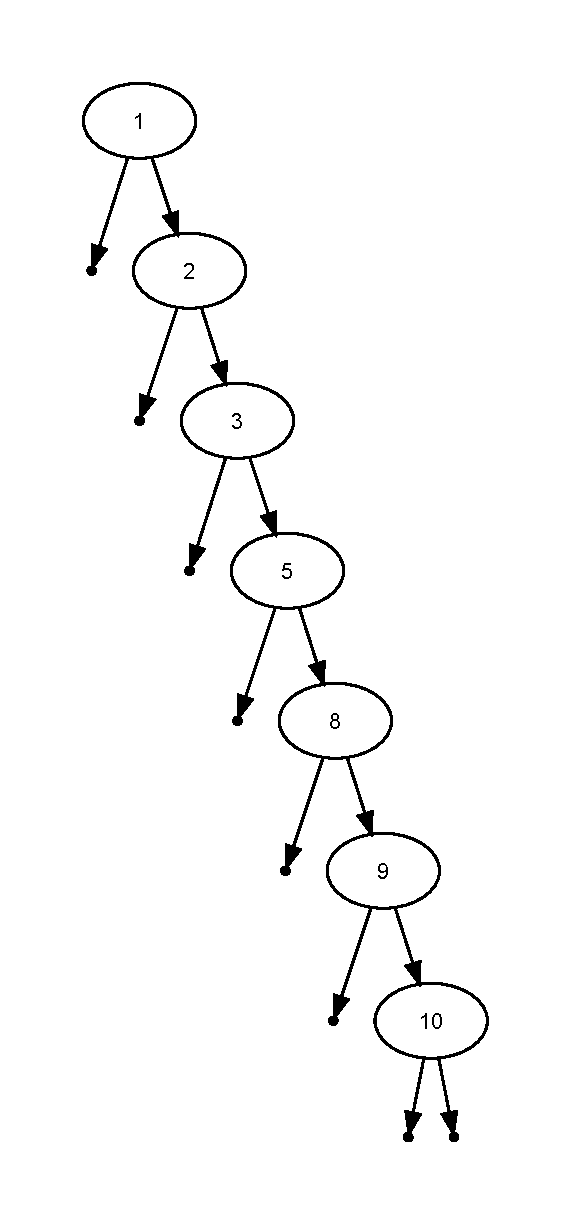
\includegraphics[width=0.5\textwidth,height=11cm]{unbalanced} \\
		(a) & (b)
	\end{tabular}
	\caption{Árboles de búsqueda binarios (a) Inserción ideal en el árbol, se logra una altura mínima y árbol completo (lleno), (b) inserción de datos ordenados, adquiere el comportamiento de una lista enlazada en donde el tiempo de búsqueda en el peor de los casos es lineal.}
	\label{fig:bst}
\end{figure}

%------------------------------------------------
\subsection{Árboles balanceados}
Uno de los primeros trabajos en abordar el problema de la inserción aleatoria en árboles binarios de búsqueda fue el de~\cite{adelson1962}; conocido también como AVL debido a los apellidos de los dos autores; su propuesta se basa en mantener un factor de balance no mayor que 1 o menor que -1, entonces después de cada operación de inserción o borrado se debe de revisar la altura de los sub-árboles izquierdo y derecho, al encontrar una violación al factor de balance los autores proponen un conjunto de rotaciones con la finalidad de balancear la altura del árbol final.
\subsubsection{Altura}
Se presenta el Algoritmo \ref{altura} para calcular la altura de un nodo. En caso de que el nodo no exista se retornará cero.

\begin{algorithm}
\caption{Cálculo la altura de un nodo}\label{altura}
\begin{algorithmic}[1]
%\Require $ a < b$ , $(f(a) < 0 $ y $f(b) > 0)$ o $(f(a) < 0$ y $f(b)) > 0$ 
%\Ensure Enésima raiz de x
\Procedure{Height}{node}
%\State $N \gets 1 $
%\While{N $\leq$ iteration}
%\State $c \gets \frac{a + b}{2}$
\If{x == NULL}
\State Return 0
%\EndIf
%$N \gets N + 1$
%\If{ \Call{Sign}{f(c)} $==$ \Call{Sign}{f(a)} }
%\State $a \gets c $
\Else 
\State Return node.height
\EndIf
%\EndWhile
\EndProcedure
\end{algorithmic}
\end{algorithm}

\subsubsection{Factor de balance}
Se define como la diferencia entre la altura del sub- árbol derecho menos la altura del sub-árbol izquierdo. Se presenta el Algoritmo \ref{factorbalance} para calcular este factor de balance.

\begin{algorithm}
\caption{Cálculo del factor de balance de un nodo}\label{factorbalance}
\begin{algorithmic}[1]
%\Require $ a < b$ , $(f(a) < 0 $ y $f(b) > 0)$ o $(f(a) < 0$ y $f(b)) > 0$ 
%\Ensure Enésima raiz de x
\Procedure{balanceFactor}{node}
%\State $N \gets 1 $
%\While{N $\leq$ iteration}
%\State $c \gets \frac{a + b}{2}$
%\If{x == NULL}
\State Return Height(node.right) - Height(node.left)
%\EndIf
%$N \gets N + 1$
%\If{ \Call{Sign}{f(c)} $==$ \Call{Sign}{f(a)} }
%\State $a \gets c $
%\Else 
%\State Return node.height
%\EndIf
%\EndWhile
\EndProcedure
\end{algorithmic}
\end{algorithm}

\subsubsection{Actualización de altura}
En cada inserción o borrado se debe de revisar la altura del sub-árbol afectado, se presenta el Algoritmo \ref{updateheight} para realizar esta tarea.
\begin{algorithm}
\caption{Revisión de la altura de un sub-árbol}\label{updateheight}
\begin{algorithmic}[1]
%\Require $ a < b$ , $(f(a) < 0 $ y $f(b) > 0)$ o $(f(a) < 0$ y $f(b)) > 0$ 
%\Ensure Enésima raiz de x
\Procedure{updateHeight}{node}
\State $HL \gets $ Height(node.left) 
\State $HR \gets $ Height(node.right) 
%\While{N $\leq$ iteration}
%\State $c \gets \frac{a + b}{2}$
\If{ HL > HR} 
\State node.height $\gets$ HL + 1
%\EndIf
%$N \gets N + 1$
%\If{ \Call{Sign}{f(c)} $==$ \Call{Sign}{f(a)} }
%\State $a \gets c $
\Else 
\State node.height $\gets$ HR + 1
\EndIf
%\EndWhile
\EndProcedure
\end{algorithmic}
\end{algorithm}

\subsubsection{Rotación derecha}
Se utiliza cuando se inserta en un sub-árbol izquierdo de otro sub-árbol, el Algoritmo \ref{rightrotation} lo detalla. Otros autores consideran un conjunto de rotaciones como rotación derecha izquierda y aún más complicadas rotación derecha izquierda derecha, algunos autores proponen que aún realizando mayores rotaciones la altura del árbol es la misma que sólo realizando rotaciones simples.  
\begin{algorithm}
\caption{Rotación derecha en un sub-árbol}\label{rightrotation}
\begin{algorithmic}[1]
%\Require $ a < b$ , $(f(a) < 0 $ y $f(b) > 0)$ o $(f(a) < 0$ y $f(b)) > 0$ 
%\Ensure Enésima raiz de x
\Procedure{RightRotation}{node}
\State temp $\gets $ node.left
\State node.left $\gets$ temp.right
\State temp.right $\gets$ node
\State updateHeight(node)
\State updateHeight(temp)
\EndProcedure
\end{algorithmic}
\end{algorithm}


\subsubsection{Rotación izquierda}
La rotación izquierda es simétrica a la rotación derecha y se origina cuando se inserta en un sub-árbol derecho de otro sub-árbol derecho. En el Algoritmo \ref{leftrotation} se describe su función.
\begin{algorithm}
\caption{Rotación izquierda en un sub-árbol}\label{leftrotation}
\begin{algorithmic}[1]
%\Require $ a < b$ , $(f(a) < 0 $ y $f(b) > 0)$ o $(f(a) < 0$ y $f(b)) > 0$ 
%\Ensure Enésima raiz de x
\Procedure{leftRotation}{node}
\State temp $\gets $ node.right
\State node.right $\gets$ temp.left
\State temp.left $\gets$ node
\State updateHeight(node)
\State updateHeight(temp)
\EndProcedure
\end{algorithmic}
\end{algorithm}


\section{Implementación}
Para la visualización del árbol AVL luego de un conjunto de operaciones se ha utilizado GraphViz\footnote{\url{http://www.graphviz.org/Home.php}}, esta biblioteca utiliza un lenguaje para la generación de grafos con nodos, se ha utilizado un método show que permita generar este código a partir de la estructura del árbol y luego desde una consola de sistema se utiliza el programa dot de Graphviz para la generación de la imagen. Ej. Para generar una imagen a partir de un archivo bstree.dot se ejecuta el siguiente comando:
\[\text{dot -Tpdf bstree.dot -o bstree.pdf}\]
La opción -T es para indicar el formato de salida de la imagen, puede ser png, jpg, pdf, etc., la opción -o es para indicar la salida del programa, en este caso se indica el nombre del formato de salida. Todas las imágenes en este documento fueron generadas son el soporte de esta herramienta.\\
Para la implementación de esta estructura se ha utilizado dos clases \textbf{avlNode} y \textbf{avlTree}, y se han implementado los métodos básicos de un árbol como insert, search, remove y algunos métodos privados como min, max y deleteMin, estos últimos sirven para alcanzar los objetivos de los primeros métodos. También debemos de resaltar que un árbol AVL posee los métodos de un árbol binario de búsqueda y adiciona algunos para el manejo de rotaciones y cálculo de la altura.\\
Implementamos nuestra clase AVLNode como sigue:
\lstinputlisting[language=c++,firstline=14,lastline=31, frame =single, basicstyle=\footnotesize,tabsize=3,keywordstyle=\color{blue},morekeywords={assert},keepspaces=true]{AVLTree.h}
También implementamos nuestro árbol AVL como:
\lstinputlisting[language=c++,firstline=33,lastline=58, frame =single, basicstyle=\footnotesize,tabsize=3,keywordstyle=\color{blue},morekeywords={assert},keepspaces=true]{AVLTree.h}
Debemos observar que para el método de eliminación de nodos se utiliza e algoritmo de Hibbard con un paso adicional sobre la revisión de alturas. Para detalles de la implementación de este código revisar el archivo AVLTree.h que acompaña este documento.
\newpage
\section{Resultados y conclusiones}
Se realizaron pruebas validando el funcionamiento de la implementación con  un conjunto de inserciones y eliminaciones, en la \figurename~\ref{fig:bstree03} presentamos el resultado de insertar las llaves 10, 8, 11, 14, 20, 3, 5, 30, 24, 16, 11, 1, 32, 21, 13, 9, 17, 27, 31, 2. en un árbol binario de búsqueda.
\begin{figure}[!h]
	\centering
	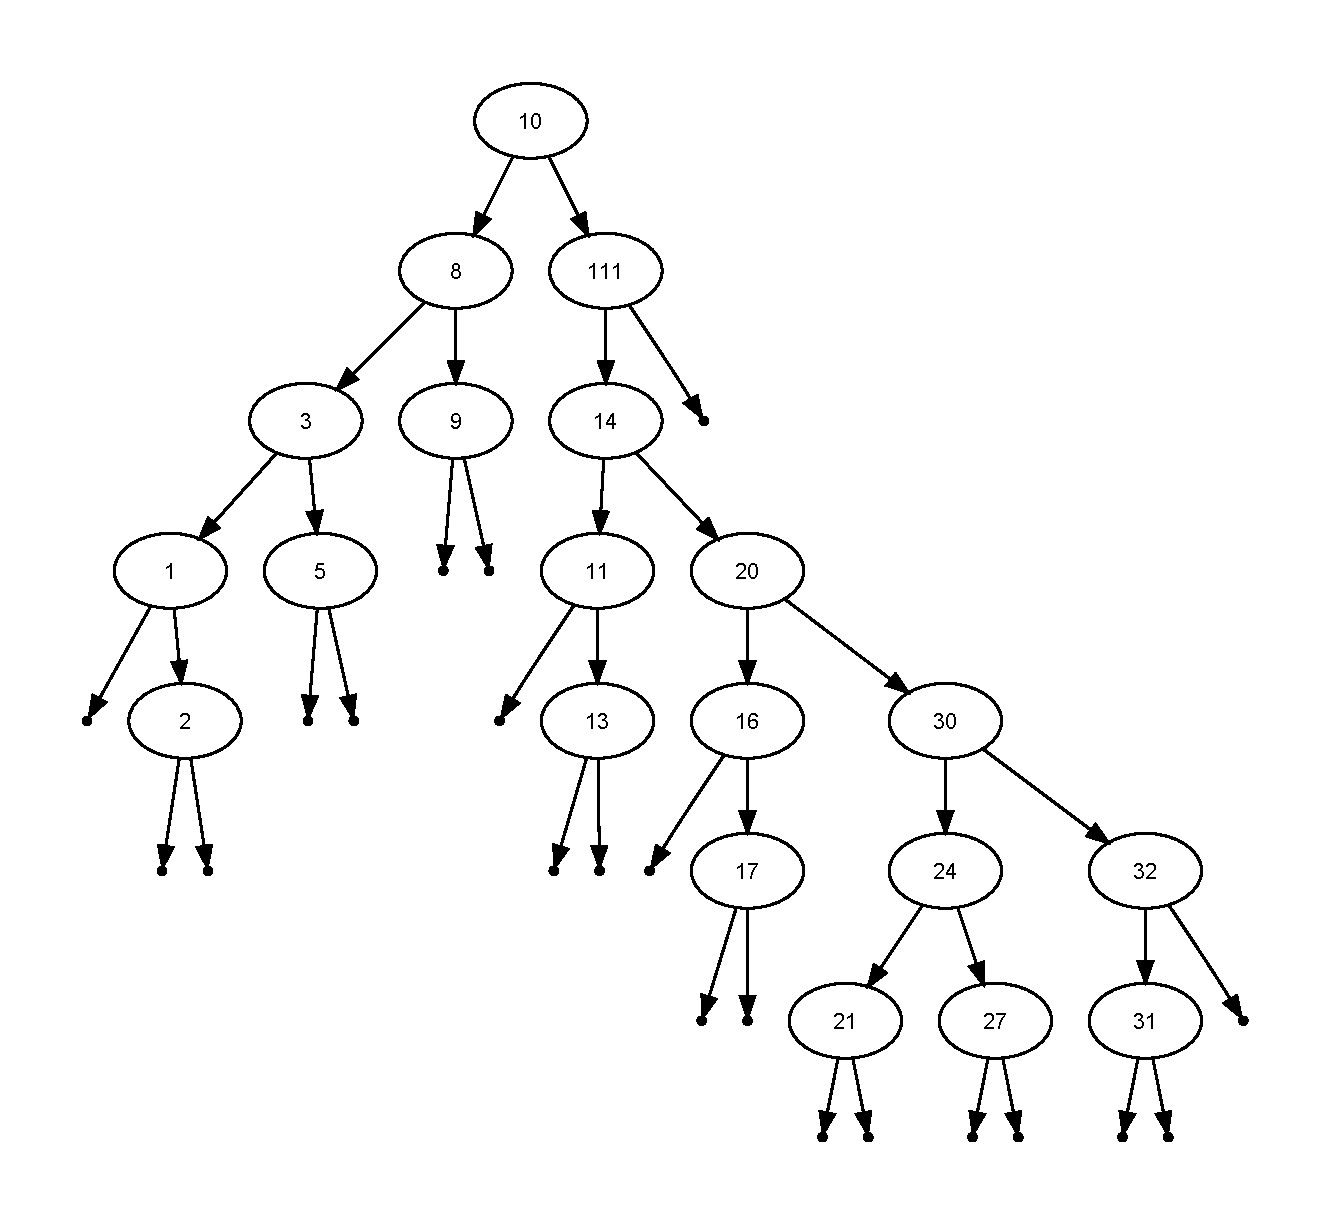
\includegraphics[width=\textwidth,height=16cm]{bstree03}	
	\caption{Inserción de llaves 10, 8, 11, 14, 20, 3, 5, 30, 24, 16, 11, 1, 32, 21, 13, 9, 17, 27, 31, 2. en un árbol binario de búsqueda}
	\label{fig:bstree03}
\end{figure}
\newpage
Luego realizamos un conjunto de eliminaciones con las siguientes llaves 20, 9, 30. y obtenemos el árbol mostrado en la \figurename~\ref{fig:bstree05}.
\begin{figure}[!h]
	\centering
	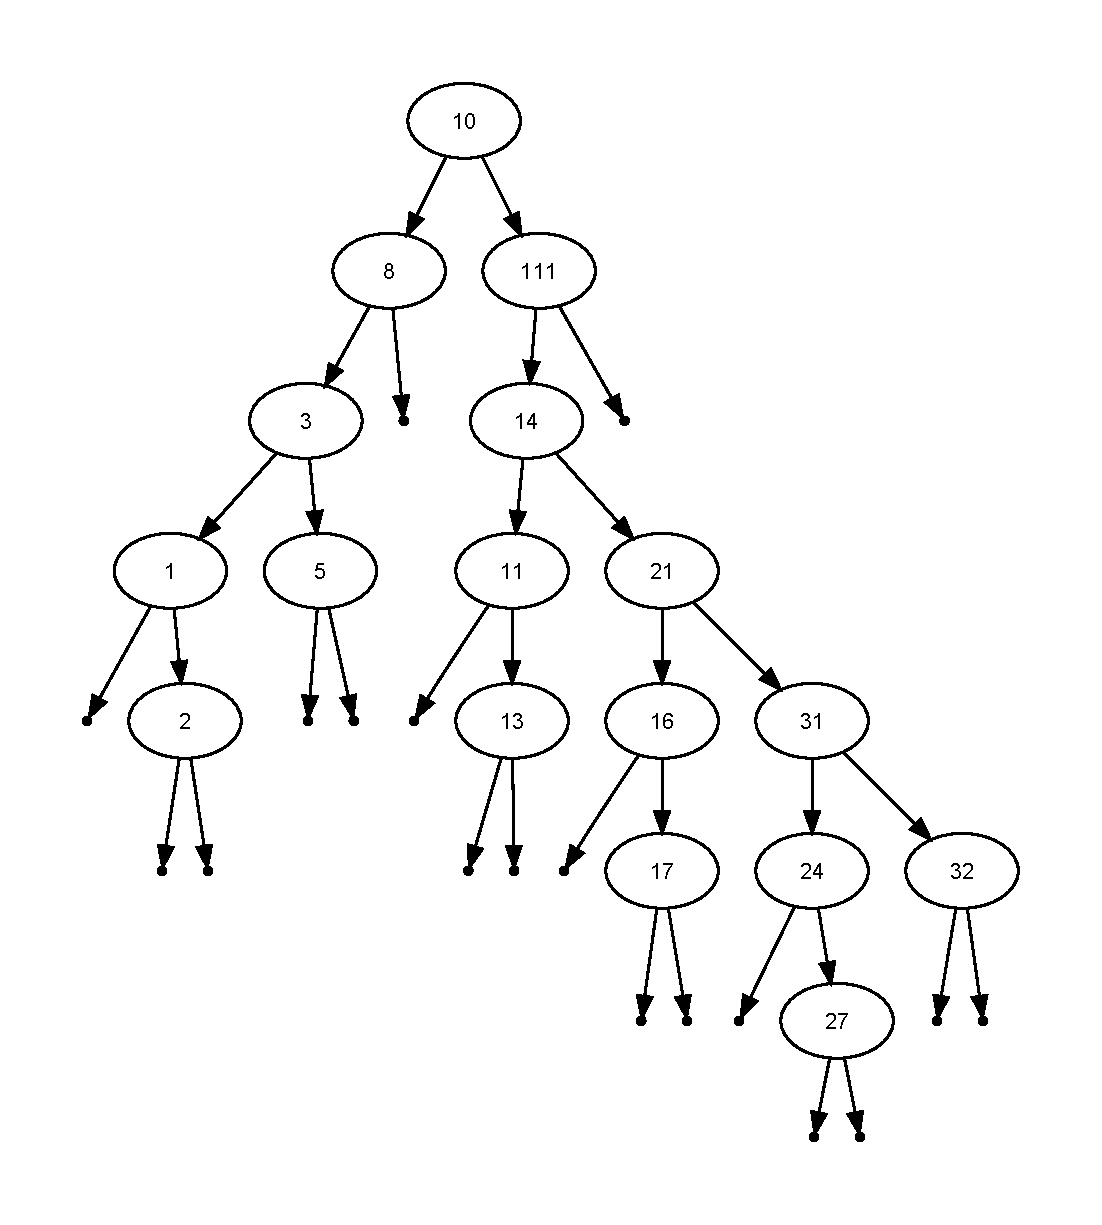
\includegraphics[width=\textwidth,height=17cm]{bstree05}	
	\caption{Árbol resultado de eliminar las llaves 20, 9, 30 en el árbol de búsqueda binaria de la \figurename~\ref{fig:bstree03}}
	\label{fig:bstree05}
\end{figure}
\newpage

También, en la \figurename~\ref{fig:avltree03} presentamos el resultado de insertar las mismas llaves pero en un árbol AVL.
\begin{figure}[!h]
	\centering
	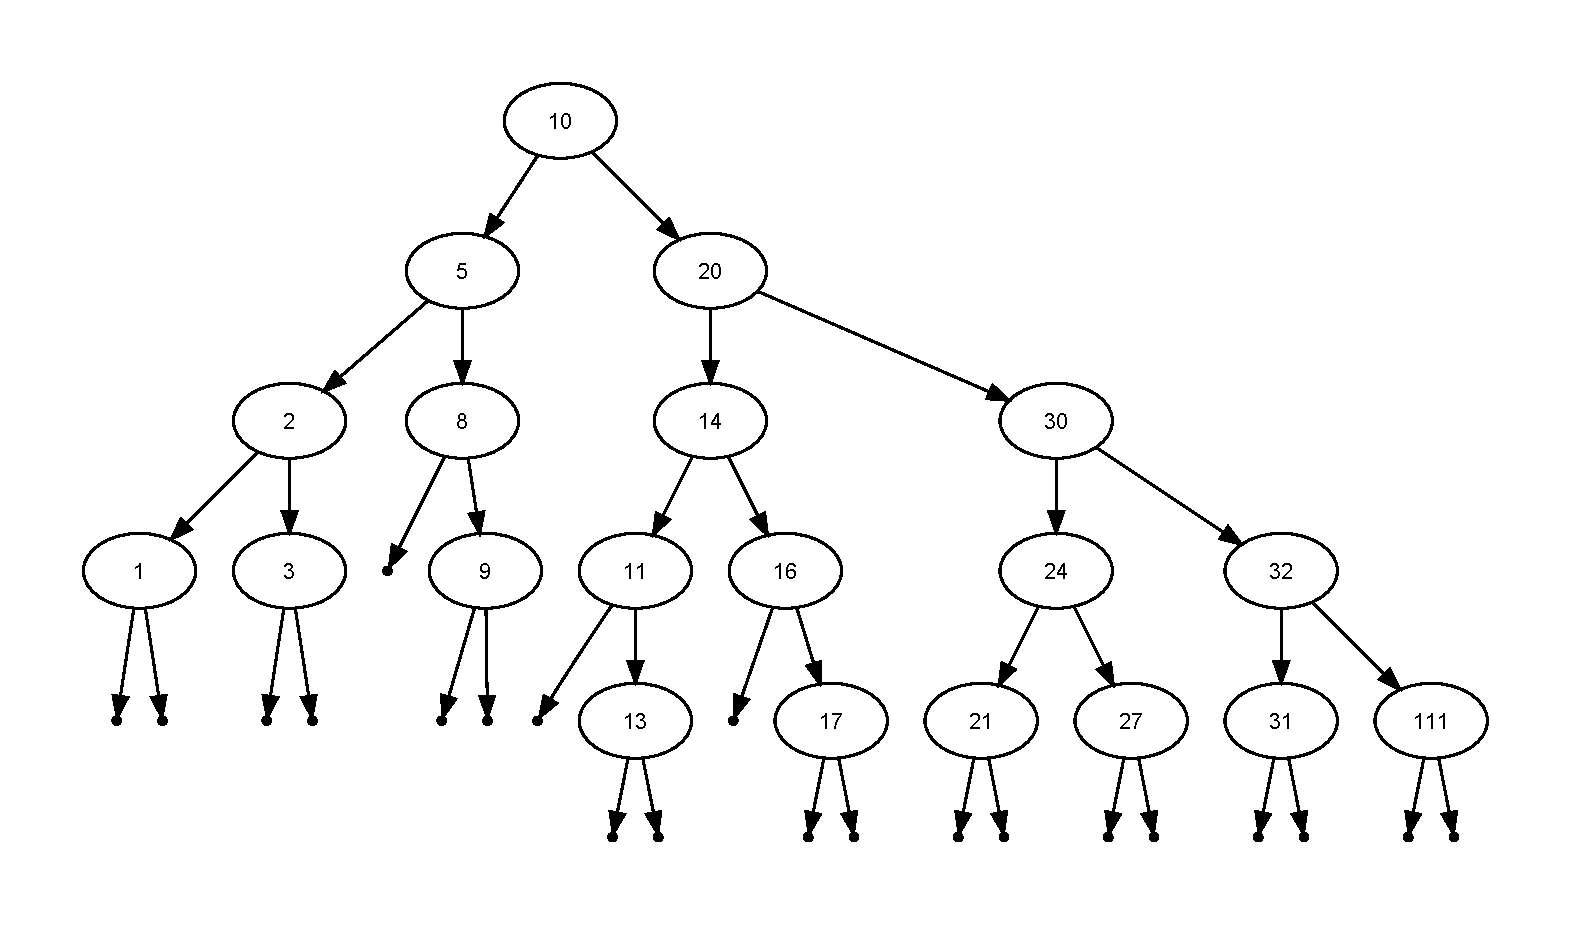
\includegraphics[width=\textwidth,height=12cm]{avltree03}
	\caption{Inserción de las llaves 10, 8, 11, 14, 20, 3, 5, 30, 24, 16, 11, 1, 32, 21, 13, 9, 17, 27, 31, 2. en un árbol AVL}
	\label{fig:avltree03}
\end{figure}
\newpage
Finalmente, en la \figurename~\ref{fig:avltree05} se presenta el resultado de eliminar las llaves 20, 9, 30 en el árbol AVL de la \figurename~\ref{fig:avltree03}.
\begin{figure}[!h]
	\centering
	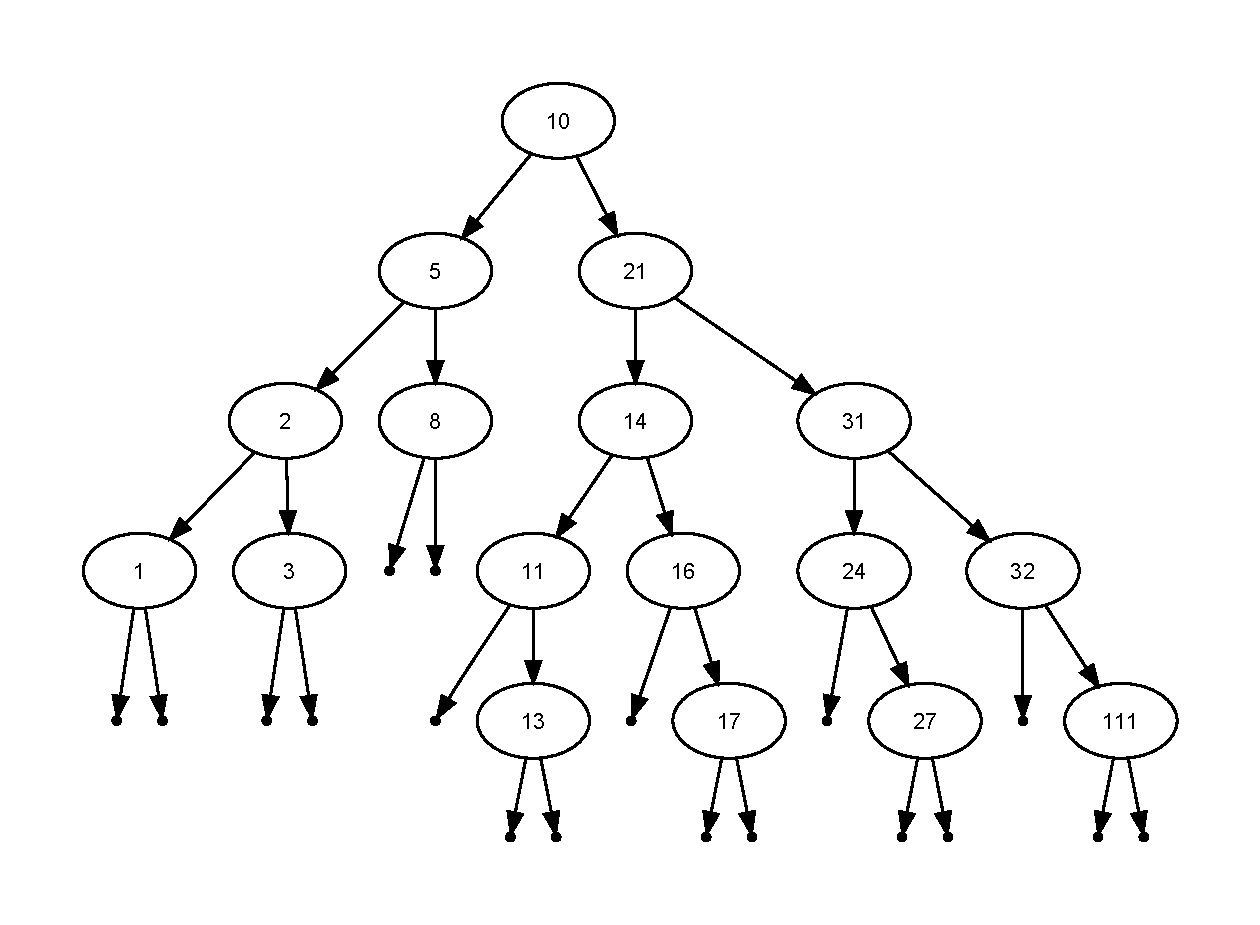
\includegraphics[width=\textwidth,height=12cm]{avltree05}
	\label{fig:avltree05}
\end{figure}
\subsection{Conclusiones} 
El árbol AVL agrega métodos para evitar el crecimiento en altura de los árboles binarios de búsqueda, se estima que mantiene su valor en $\sim 1.44 \ln N$. Existen un conjunto de rotaciones que ayudan a mantener la altura, pero se logran buenos resultados utilizando las rotaciones básicas a la derecha e izquierda. \\Existen otros árboles como el árbol rojo-negro que considera otros factores que permiten obtener tiempos logarítmicos en inserción y búsqueda, sin embargo el árbol AVL permite sustentar las bases de estos algoritmos más avanzados.

\bibliographystyle{apalike}

\begin{thebibliography}{2}
   \bibitem{adelson1962}
  \textit{An information organization algorithm},
  Adelson-Velskii, Georgy Maximovic and Landis, Evgenii Mikhailovich,
  Doklady Akademia Nauk SSSR,
  vol. 146,
  pag. 263--266,
  1962	
  \bibitem{reed2000}
  \textit{How tall is a tree?},
  Reed, Bruce,
  Proceedings of the thirty-second annual ACM symposium on Theory of computing,
  pag. 479--483,
  ACM,
  2000
  
\end{thebibliography}

\end{document}